\section{Singleton Move} % (fold)
\label{sec:singleton_move}

    La prima mossa che si è scelto di implementare è la Singleton Move. Il \textit{contorno} di una tile è definito come in figura \ref{fig:singleTile}, ovvero consiste dell'insieme di tiles adiacenti alla tile corrente rispetto ai quattro punti cardinali. Una \textit{copertura} è un insieme di tiles posizionate nella board in modo che nessuna di queste tile sia posizionata nel contorno di un'altra. Una \textit{copertura massimale} è una copertura di cardinalità massima, ovvero: aggiungendo una qualsiasi tile, tale insieme non è più una copertura. Un esempio di copertura massimale è raffigurato in figura \ref{fig:maximal_cover}.

    \begin{figure}[H]
		\centering
		\begin{minipage}{.5\textwidth}
  			\begin{figure}[H]
                \centering
                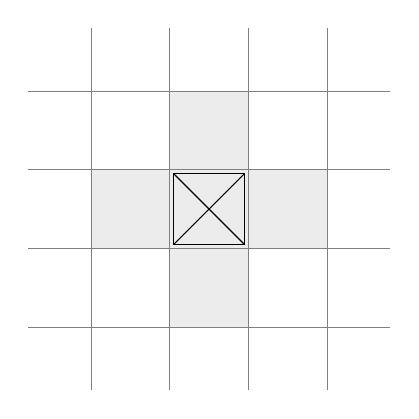
\begin{tikzpicture}
                    \foreach \x/\y in {2/2}
                    {
                        \fill[fill=gray!15!white] (\x,\y) rectangle (\x+1,\y+1);
                        \fill[fill=gray!15!white] (\x+1,\y) rectangle (\x+2,\y+1);
                        \fill[fill=gray!15!white] (\x,\y+1) rectangle (\x+1,\y+2);
                        \fill[fill=gray!15!white] (\x-1,\y) rectangle (\x,\y+1);
                        \fill[fill=gray!15!white] (\x,\y-1) rectangle (\x+1,\y);
                        \draw[black] (\x+.05,\y+.05) rectangle (\x+.95,\y+.95);
                        \draw[black] (\x+.05,\y+.05) -- (\x+.95,\y+.95);
                        \draw[black] (\x+.95,\y+.05) -- (\x+.05,\y+.95);
                    }
                    \draw[step=1cm,gray,very thin] (.2,.2) grid (4.8,4.8);
                \end{tikzpicture}
                \caption{Single tile selection}
                \label{fig:singleTile}
    		\end{figure}
		\end{minipage}%
		\begin{minipage}{.5\textwidth}
			\begin{figure}[H]
            \centering
            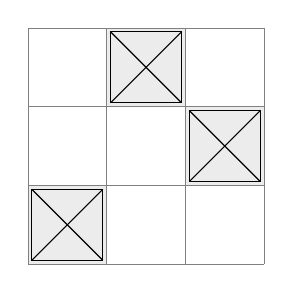
\begin{tikzpicture}
                \foreach \x/\y in {0/0,1/2,2/1}
                {
                    \fill[fill=gray!15!white] (\x,\y) rectangle (\x+1,\y+1);
                    \draw[black] (\x+.05,\y+.05) rectangle (\x+.95,\y+.95);
                    \draw[black] (\x+.05,\y+.05) -- (\x+.95,\y+.95);
                    \draw[black] (\x+.95,\y+.05) -- (\x+.05,\y+.95);
                }
                \draw[step=1cm,gray,very thin] (0,0) grid (3,3);
            \end{tikzpicture}
            \caption{Maximal cover of single tiles}
            \label{fig:maximal_cover}
    		\end{figure}
		\end{minipage}
	\end{figure}


    

    


    La SingletonMove consiste nei seguenti passi:
    \begin{itemize}
    	\item[1.] prende una copertura massimale in modo random, garantendo che tale scelta sia \textbf{unbiased}. In questa fase, un vettore $coords$ di coordinate viene creato, corrispondente alle coordinate delle tile scelte nella board. 
    	\item[2.] crea un vettore di \textbf{coppie} di interi $permutation$ lungo tanto quanto il numero di tile selezionate. La semantica è la seguente: la mossa sceglie di spostare la tile che si trovava in coordinata $coords[permutation[i].first]$ nella coordinata $coords[i]$ con orientamento $permutation[i].second$.
    	\item[3.] sceglie (in modo random o tramite la First e la Next) una permutazione del vettore $permutation$ e applica la mossa (si veda il metodo \texttt{MakeMove(\dots)}).
    \end{itemize}

    Analizziamo il primo passo: la selezione delle coordinate random avviene nello stato. Come già detto nell'overview, questa scelta è stata fatta perchè si è voluto rigenerare l'insieme di coordinate dopo un certo numero di applicazioni random di tale mossa e perchè, nel momento in cui si chiami \texttt{BestMove(\dots)} si arriva subito ad un ottimo locale di questa mossa: questo necessita di una rigenerazione delle mosse. In questo senso, la mossa risulta \textbf{parametrizzata} dal vettore delle coordinate scelte. Il passo $1$ è implementato dalla funzione \texttt{singletonRandomCoords(\dots)}: viene scelta una coordinata random in modo totalmente unbiased, cioè scegliendo random due numeri nel range $[1 \dots board.size]$, e viene controllata la sua feasibility testando se corrisponde al contorno di un'altra tile: in tal caso, viene ripetuta la generazione di una coordinata. Il ciclo si ferma quando tutte le celle della board sono state coperte da una tile o dal contorno di una tile, ottenendo quindi una \textit{copertura massimale}. Il vantaggio di questa funzione è che genera una copertura massimale in modo unbiased; lo svantaggio è che nelle ultime iterazioni del ciclo, potrebbe essere il caso che scarti molte volte la coordinata generata in quanto infeasible e che quindi ci vogliano molte iterazioni per arrivare alla massimalità.

    Tale generazione delle coordinate è stata scelta perchè consente di calcolare il $\Delta$-costo in maniera molto efficacie: il $\Delta$-costo di tale mossa viene calcolato sommando i $\Delta$-costi di tutte le tile spostate. A sua volta, il $\Delta$-costo di una singola tile è molto facile da calcolare, in quanto basta prendere la tile, spostarla nella coordinata prevista dalla mossa con il rispettivo orientamento e ciclare per tutti e quattro i punti cardinali: se il bordo della tile non coincide con il bordo della tile presente nella board in tale direzione, allora si somma $1$ al costo. Si noti come questo semplice algoritmo si complicherebbe di molto nel caso in cui non considerassimo il \textit{contorno} di ogni tile.

    Nel secondo passo, la mossa prende coscienza delle coordinate sulle quali si baseranno tutti i suoi metodi: questo passo è implementato nelle funzioni \texttt{FirstMove(\dots)} e \texttt{RandomMove(\dots)}, tramite i seguenti metodi:
    \begin{itemize}
    	\item \texttt{mv.setCoordinates(st.random\_singleton)}: imposta il vettore delle coordinate $coords$ della mossa prendendo tali coordinate dallo stato
    	\item \texttt{mv.createPermutationVector(st.random\_singleton.size())}: crea il vettore $permutation$ della giusta grandezza, i.e. $board.size$.
    \end{itemize}

    Infine, analizziamo il terzo passo. Il vettore $permutation$ viene riempito in modo diverso a seconda di quale funzione della mossa si chiami:
    \begin{itemize}
    	\item La \textit{FirstMove} setta $permutation$ al vettore identico e tutti gli orientamenti a $0$, i.e. $permutation[i] = (i,0) \ \forall i$: questo perchè la prima mossa dell'intorno è la mossa che rimette tutte le tiles nelle posizioni originali con orientamento $0$.
    	\item La \textit{NextMove} calcola la prossima permutazione nel seguente modo. Sia $\pi_0$ la proiezione del vettore $permutation$ sulla prima componente, i.e.: $\pi_0[i] = permutation[i].first$ e sia $\pi_1$ la proiezione del vettore $permutation$ sulla seconda componente, i.e.: $\pi_1[i] = permutation[i].second$. La \textit{NextMove} considera $\pi_1$ come un numero in base $4$ e lo incrementa. Se $\pi_1[i] = 3 \ \forall i$, allora incrementa il vettore $\pi_0$ con il classico metodo per calcolare la prossima permutazione ed setta $\pi_1[i] = 0 \ \forall i$. Infine imposta $permutation[i].first = \pi_0[i]$ e $permutation[i].second = \pi_1[i]$, modificando quindi correttamente la mossa. Un esempio di applicazione della \textit{NextMove} è raffigurato in figura \ref{fig:next_example}.

    	\begin{figure}[H]
            \centering
            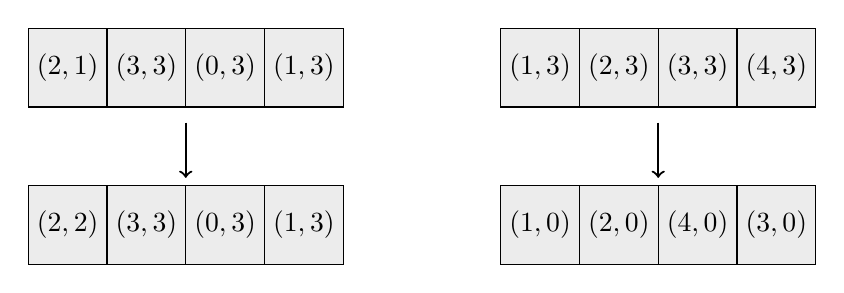
\begin{tikzpicture}
            	\foreach \x/\y in {0/0,1/0,2/0,3/0}
                {
                    \fill[fill=gray!15!white,draw=black] (\x,\y) rectangle (\x+1,\y+1);
                    \fill[fill=gray!15!white,draw=black] (\x,\y) rectangle (\x+1,\y+1);

                    \fill[fill=gray!15!white,draw=black] (\x,\y+2) rectangle (\x+1,\y+3);
                    \fill[fill=gray!15!white,draw=black] (\x,\y+2) rectangle (\x+1,\y+3);

                    \fill[fill=gray!15!white,draw=black] (\x+6,\y) rectangle (\x+7,\y+1);
                    \fill[fill=gray!15!white,draw=black] (\x+6,\y) rectangle (\x+7,\y+1);

                    \fill[fill=gray!15!white,draw=black] (\x+6,\y+2) rectangle (\x+7,\y+3);
                    \fill[fill=gray!15!white,draw=black] (\x+6,\y+2) rectangle (\x+7,\y+3);
                }

                \node at (0.5,2.5) {$(2,1)$};
                \node at (1.5,2.5) {$(3,3)$};
                \node at (2.5,2.5) {$(0,3)$};
                \node at (3.5,2.5) {$(1,3)$};

                \node at (0.5,0.5) {$(2,2)$};
                \node at (1.5,0.5) {$(3,3)$};
                \node at (2.5,0.5) {$(0,3)$};
                \node at (3.5,0.5) {$(1,3)$};

                \node at (6.5,2.5) {$(1,3)$};
                \node at (7.5,2.5) {$(2,3)$};
                \node at (8.5,2.5) {$(3,3)$};
                \node at (9.5,2.5) {$(4,3)$};

                \node at (6.5,0.5) {$(1,0)$};
                \node at (7.5,0.5) {$(2,0)$};
                \node at (8.5,0.5) {$(4,0)$};
                \node at (9.5,0.5) {$(3,0)$};

                \draw[thick,black,->] (2.0,1.8) -- (2.0,1.1);
                \draw[thick,black,->] (8.0,1.8) -- (8.0,1.1);
            \end{tikzpicture}
            \caption{Two examples of NextMove execution.}
            \label{fig:next_example}
    	\end{figure}

    	\item La \textit{RandomMove} calcola una permutazione random delle coordinate e degli orientamenti in modo totalmente unbiased: questo è stato garantito dall'implementazione dell'algoritmo \textit{Fisher and Yates Shuffle}, che crea una permutazione casuale degli elementi, creando quindi $\pi_0$. Gli orientamenti (i.e. $\pi_1$) invece vengono generati semplicemente scegliendo un numero random nell'intervallo $[0,3]$.
    \end{itemize}


    Sia $n$ il numero di coordinate scelte per tale mossa: l'intorno della SingletonMove ha cardinalità $3^n n!$, chiaramente esponenziale. Per questo motivo la \textit{BestMove} (nel codice \texttt{SelectBest(\dots)}) è stata implementata tramite l'\textbf{Hungarian ALgorithm}, che trova il minimo matching in un grafo bipartito pesato completo. La \textit{BestMove} crea quindi tale grafo $G=(U,V,E)$, dove $U=V=\{1 \dots n\}$ e:
    \begin{center}
    $E = \{ (i,j) \ | \ i \in U , j \in V , w(i,j) = $ minimo costo di mettere in posizione $coords[j]$ la tile che era in posizione $coords[i]$ \\ fra tutti gli orientamenti possibili $\}$
    \end{center}
    La matrice di adiacenza di $G$ è quindi tale che $G[i,j] = (w(i,j),r)$, dove $w(i,j)$ è il peso dell'arco ed $r$ è l'orientamento minimo di cui prima. Un esempio di grafo generato è raffigurato in figura \ref{fig:graph_hungarian}: il matching di costo minimo è $M=\{(0,0),(1,2),(2,1)\}$. 

    	\begin{figure}[H]
            \centering
            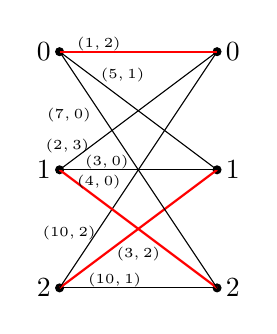
\begin{tikzpicture}
            	\foreach \x/\y in {0/0,2/0}
                {
                    \draw[fill=black] (\x,\y) circle [radius = 0.05];
                    \draw[fill=black] (\x,\y+1.5) circle [radius = 0.05];
                    \draw[fill=black] (\x,\y+3) circle [radius = 0.05];
				}

				\node at (-0.2,0.0) {$2$};
				\node at (-0.2,1.5) {$1$};
				\node at (-0.2,3.0) {$0$};

				\node at (2.2,0.0) {$2$};
				\node at (2.2,1.5) {$1$};
				\node at (2.2,3.0) {$0$};

				\draw[black] (0,0) -- (2,0); \node at (0.12,0.7) {\tiny $(10,2)$};
				\draw[red,thick] (0,0) -- (2,1.5); \node at (1.0,0.43) {\tiny $(3,2)$};
				\draw[black] (0,0) -- (2,3); \node at (0.7,0.1) {\tiny $(10,1)$};

				\draw[red,thick] (0,1.5) -- (2,0); \node at (0.1,1.8) {\tiny $(2,3)$};
				\draw[black] (0,1.5) -- (2,1.5); \node at (0.6,1.6) {\tiny $(3,0)$};
				\draw[black] (0,1.5) -- (2,3); \node at (0.5,1.35) {\tiny $(4,0)$};

				\draw[black] (0,3) -- (2,0); \node at (0.12,2.2) {\tiny $(7,0)$};
				\draw[black] (0,3) -- (2,1.5); \node at (0.8,2.7) {\tiny $(5,1)$};
				\draw[red,thick] (0,3) -- (2,3); \node at (0.5,3.1) {\tiny $(1,2)$};
               
            \end{tikzpicture}
            \caption{Graph for the Hungarian Algorithm.}
            \label{fig:graph_hungarian}
    	\end{figure}

    Tramite il mathing minimo e il vettore delle coordinate $coords$, la \textit{BestMove} è in grado di costruire la mossa ottima nell'intorno. In generale, la mossa sposterà la tile che si trovava in posizione $coords[match[i].first]$ in posizione $coords[match[i].second]$ con rotazione $G[match[i]].second$.

    Dato che l'Hungarian Algorithm è polinomiale nella grandezza del grafo e dato che il grafo ha $2n$ nodi, la \textit{BestMove} riesce a scegliere la mossa migliore in tempo polinomiale, mentre una versione naive che chiama \textit{First} e \textit{Next} avrebbe costo esponenziale.

    Come ultima osservazione, si noti come la SingletonMove generalizzi le seguenti mosse:
    \begin{itemize}
    	\item[1.] la mossa che sposta (con eventuale rotazione) due singole tile prese il modo random dalla board
    	\item[2.] le mosse EvenChessboard e OddChessboard, in quanto entrambe si basano su un insieme di coordinate che è una copertura massimale
    \end{itemize}

    Tutte le osservazioni fatte in questa sezione ad eccezione della generazione random delle coordinate si ripetono per tutte le altre mosse: questo giustifica la trattazione approfondita che si è tenuta in questa sezione.

% section singleton_move (end)